\documentclass{jsarticle}

\usepackage{listings,jlisting}
\usepackage[dvipdfmx]{graphicx}
\usepackage{bmpsize}
\usepackage{bm}

\lstset{
    basicstyle={\ttfamily},
    identifierstyle={\small},
    commentstyle={\smallitshape},
    keywordstyle={\small\bfseries},
    ndkeywordstyle={\small},
    stringstyle={\small\ttfamily},
    frame={tb},
    breaklines=true,
    columns=[l]{fullflexible},
    numbers=left,
    xrightmargin=0zw,
    xleftmargin=3zw,
    numberstyle={\scriptsize},
    stepnumber=1,
    numbersep=1zw,
    lineskip=-0.5ex
}
\begin{document}

\title{計算機科学実験及演習4 エージェント 課題3}
\author{1029-28-2473 二見 颯}
\maketitle

\section{プログラム概要}
サポートベクター回帰を実装して、その性能を交差検証によって評価した。 \\
また、リスティングデータ(San Francisco)から民泊における価格の予測を行った。

\section{外部仕様}
\begin{itemize}
    \item dat\_main.py - dat データを SVR によって予測する
    \item sanfrancisco\_main.py - SanFrancisco データセットを扱い、GridSearch によるハイパーパラメータ最適化まで行う
    \item svr.py - SVR を実装する
    \item svr\_test.py - SVRegressor の回帰式を plot して確認する
    \item utils.py - load\_data, cross\_val\_regression を実装する 
    \item scaler.py - MinMaxScaler(正規化), StandardScaler(標準化)のクラスを実装
\end{itemize}
プログラムの実行は dat\_main.py では、\\
{\bf ./dat\_main.py [入力ファイルへのパス] [param c] [param eps] [-n or -p or -g] ([param kernel])} \\ 
sanfrancisco\_main.py では、{\bf ./sanfrancisco\_main.py} とする。 \\
以下は dat\_main.py の実行例である。
\begin{lstlisting}
$ ./dat_main.py data/sample10.dat 1000.0 0.1 -g 2.236
cvxopt.solvers.qp: optimization succeeded
alpha: 
0 [1.11573444e-07]
1 [6.99586467e-08]
2 [5.90636469e-08]
3 [4.70242227e-08]
4 [3.70005294e-08]
5 [50.06320139]
6 [3.33900983e-08]
7 [3.6030674e-08]
8 [3.56733185e-08]
9 [2.78326474e-08]
alpha*: 
0 [3.12193596e-07]
1 [1.75474404e-07]
2 [1.19863781e-07]
3 [1.52689385e-07]
4 [3.4347422e-07]
5 [3.51526892e-08]
6 [50.06318089]
7 [2.53792954e-06]
8 [1.61443468e-06]
9 [1.56667801e-05]
biases candidates:  [-1.0588922598948347, -1.0588922601870785]
prediction and correct y
0.1347791896233308 0.136701623063
0.37540034444014525 0.382683432365
0.6517209209502615 0.64944804833
0.8934158368122316 0.852640164354
1.0487272722375427 0.972369920398
1.0939080552261236 1.19390805508
1.0238795323648806 0.923879532511
0.8468469018565519 0.7604059656
0.5919993050229668 0.522498564716
0.31680988727896464 0.233445363856
\end{lstlisting}

\section{内部仕様}
課題1, 2との差分を報告する。
\subsection*{SVRegressorクラス(svr.py)}
SVR(Support Vector Regression) を実装する
\begin{itemize}
    \item X, y - 訓練データ
    \item n - 訓練データの個数
    \item kf - kernel trickとして用いる関数(kernel function)
    \item p - kernel functionのパラメータ
    \item C, eps - SVR のパラメータ
    \item a, b - SVR の内部パラメータ。\_setLagrange 関数で決定する
    \item bias - SVR の内部パラメータ。\_setClassifier 関数で決定する
\end{itemize}
コンストラクタにより、kf, p, C, eps を決定する
\subsection*{fit}
X, y, nを決定して、a, b および bias を決定する各関数を呼び出す
\subsection*{\_setLagrange}
以下の2次計画問題をcvxopt.solvers.qpを用いて解くことで、a および b を決定する
\begin{eqnarray*}
\max (- \frac{1}{2} \sum_{k=0} \sum_{l=0} (a_k - b_k) (a_l - b_l) K(\bm{x_k}, \bm{x_l})
- \epsilon \sum_{k=0} (a_k + b_k) + \sum_{k=0} y_k (a_k - b_k)) \\
(\sum_{k=0} (a_k - b_k) = 0, 0 \leq a_k, b_k \leq C)
\end{eqnarray*}

\subsection*{\_setClassifier}
a, b と X, y から bias を決定する。 \\
$0 < a_i < C$を満たすデータ点について、bias$ = -y_n + \epsilon + \sum_{k=0} (a_k - b_k) (\bm{x_i}, \bm{x_k})$, \\
$0 < b_i < C$を満たすデータ点について、bias$ = -y_n - \epsilon + \sum_{k=0} (a_k - b_k) (\bm{x_i}, \bm{x_k})$によって
bias を求める(これらは全て一致する)。誤差を考慮して、$0.01C < a_i < 0.99C$ とした。

\subsection*{predict}
与えられた $X$ (バッチ入力可能)に対して、回帰式 $f(X)$ の結果を返す。\\
bias$ = \theta$として、各$x$に対して、
\begin{eqnarray*}
f(\bm{x}) = \sum_{k=0} (a_k - b_k) K(\bm{x_k}, \bm{x}) - \theta
\end{eqnarray*}

\subsection*{score}
tX に対して predict を行い、その結果と tY を比べてモデルを評価する。\\
評価基準として、引数 mth に 'MSE'(平均二乗誤差), 'MAE'(平均絶対誤差), 'R2(決定係数)'を
指定することができる。予測値を$\hat{y_i}$とすると、
\begin{eqnarray*}
MSE = \frac{1}{n} \sum_{i=0} (y_i - \hat{y_i})^2 \\
MAE = \frac{1}{n} \sum_{i=0} \| y_i - \hat{y_i} \| \\
R2 = 1 - \frac{\sum_{i=0} (y_i - \hat{y_i})^2}{\sum_{i=0} (y_i - \bar{y_i})^2}
\end{eqnarray*}

\subsection*{StandardScaler クラス(scaler.py)}
データの標準化を行う \\
fit で与えられたデータの平均、標準偏差をそれぞれ mean, std に代入して、
transform で X = (X - mean) / std と変換したXを返す。

\subsection*{sanfrancisco\_main.py}
San Francison-listings.csv を読み込んで、データの前処理を施した後に
パラメータp, Cについて Grid Search を行い最適なパラメータを求める。(モデルの
評価は交差検証によって行う) \\
データについては、95の説明変数(特徴量)のうち、'latitude', 'longitude', 'accomodates', 'property\_type', 
'room\_type', 'number\_of\_reviews', 'review\_scores\_rating'を用いる。
目的変数は 'price' とする。また、データの個数はランダムにサンプリングした500個とする。 \\
これらの選択した特徴量について、'review\_scores\_rating' には欠損値が含まれているため0へ変換した。
'room\_type', 'property\_type' のカテゴリデータについては one-hot vector 表現に直す。
これにより、n種類のカテゴリに対して、n-1種類の特徴量が新たに生成される。\\
以上の前処理を終えた後にGridSearchを実行する。

\section{評価結果}
\subsection{回帰式の確認}
sample10.dat, sample40.dat について、線形、非線形SVRで2次計画問題が正しく解けていることを確認したが、
その結果については省略する。 \\
1次元の説明変数による回帰を、実装した linear, 多項式カーネル, Gauss カーネル SVR および scikit-learn による Gauss カーネル SVR
に対して学習して、学習したものと同じデータを用いて予測した。 \\
http://scikit-learn.org/stable/auto\_examples/svm/plot\_svm\_regression.html\#sphx-glr-auto-examples-svm-plot-svm-regression-py
を参考にして、svr\_test.py を実装した。パラメータは以下の通り。
\begin{lstlisting}
svr_rbf = SVRegressor(ker_type='-g', p=1.0, c=1e3, eps=0.1)
svr_lin = SVRegressor(ker_type='-n', p=0.1, c=1e3, eps=0.1)
svr_poly = SVRegressor(ker_type='-p', p=2, c=1e3, eps=0.1)

# scikit-learn による SVR
svr_sk = SVR(kernel='rbf', gamma=1.0, C=1e3, epsilon=0.1)
\end{lstlisting}
\begin{figure}[!h]
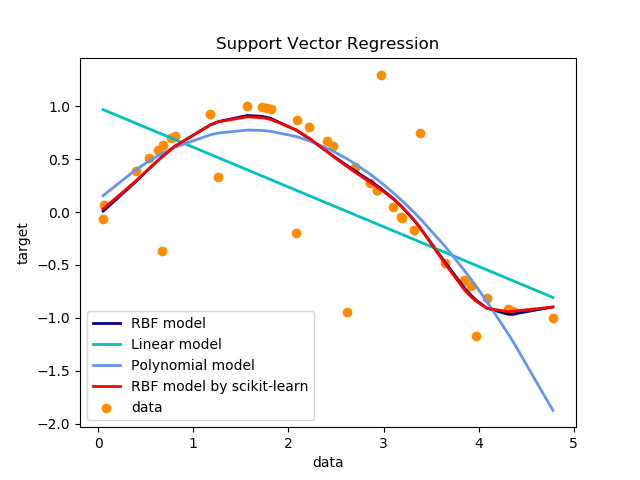
\includegraphics[width=15cm]{svr_verify.png}
\caption{verify SVR}
\end{figure}

\subsection{交差検証によるパラメータ探索(リスティングデータを用いる)}
決定係数(R2 score) によってモデルを評価した。
$c = [10.0, 100.0, 1000.0, 10000.0]$および$\sigma=[2^{-2}, 1, 2^2, 2^4, 2^6, 2^8]$の範囲で
Grid Searchした結果、決定係数が最大となったのは、$c=100.0, \sigma=4.0$の場合で、決定係数は0.4934であった。
\begin{figure}[!h]
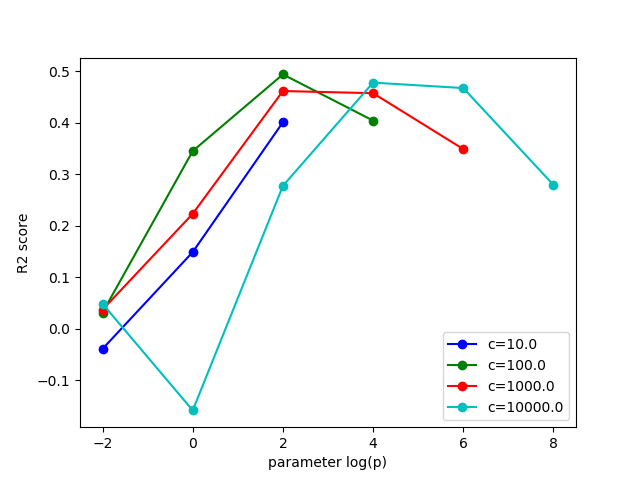
\includegraphics[width=15cm]{grid_sanfrancisco.png}
\caption{grid search about SanFrancisco}
\end{figure}
ただし、図2上で plot されていない$(c, \sigma)$ の組では、2次計画問題の後にサポートベクターが見つからず、
SVR が機能していない。

\section{考察}
% SVR の式の意味(特に c, eps について)

% 評価関数

% SanFrancisco data に関する考察
SanFrancisco data の 'price'の値について、最大値9000.0, 最小値0.0, 平均213.65で、
図3の通り、2000以降の高価格帯にはデータ数は少なく外れ値と考える方がよい。そのため、モデルの訓練および
評価には500以下のデータのみを用いることとした。
\begin{figure}[!h]
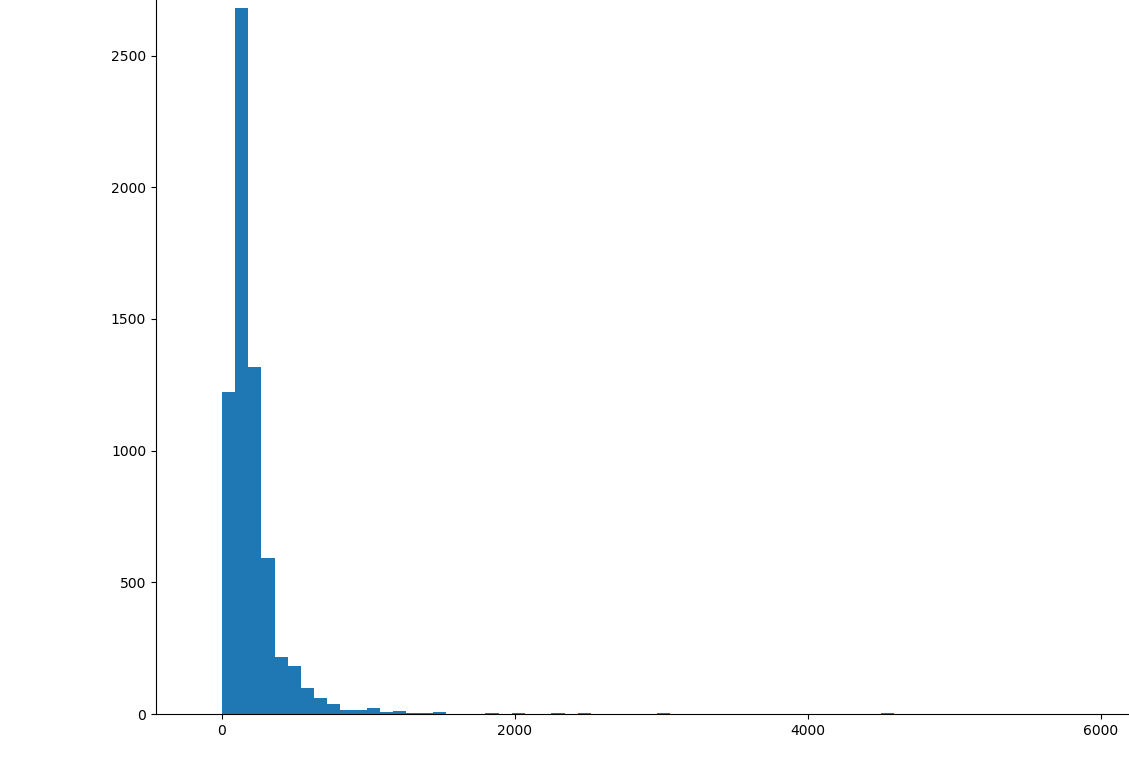
\includegraphics[width=18cm]{prices.png}
\caption{SanFrancisco price}
\end{figure}

\section{参考資料}
\begin{itemize}
    \item scikit-learn と Tensorflow による実践機械学習 Aurelien Geron 著
\end{itemize}

\end{document}
